\section{Project Management}
\subsection{Team Organization}
See figure \ref{fig:orgchart} for the team organizational chart.

\begin{figure}[htbp]
\begin{center}
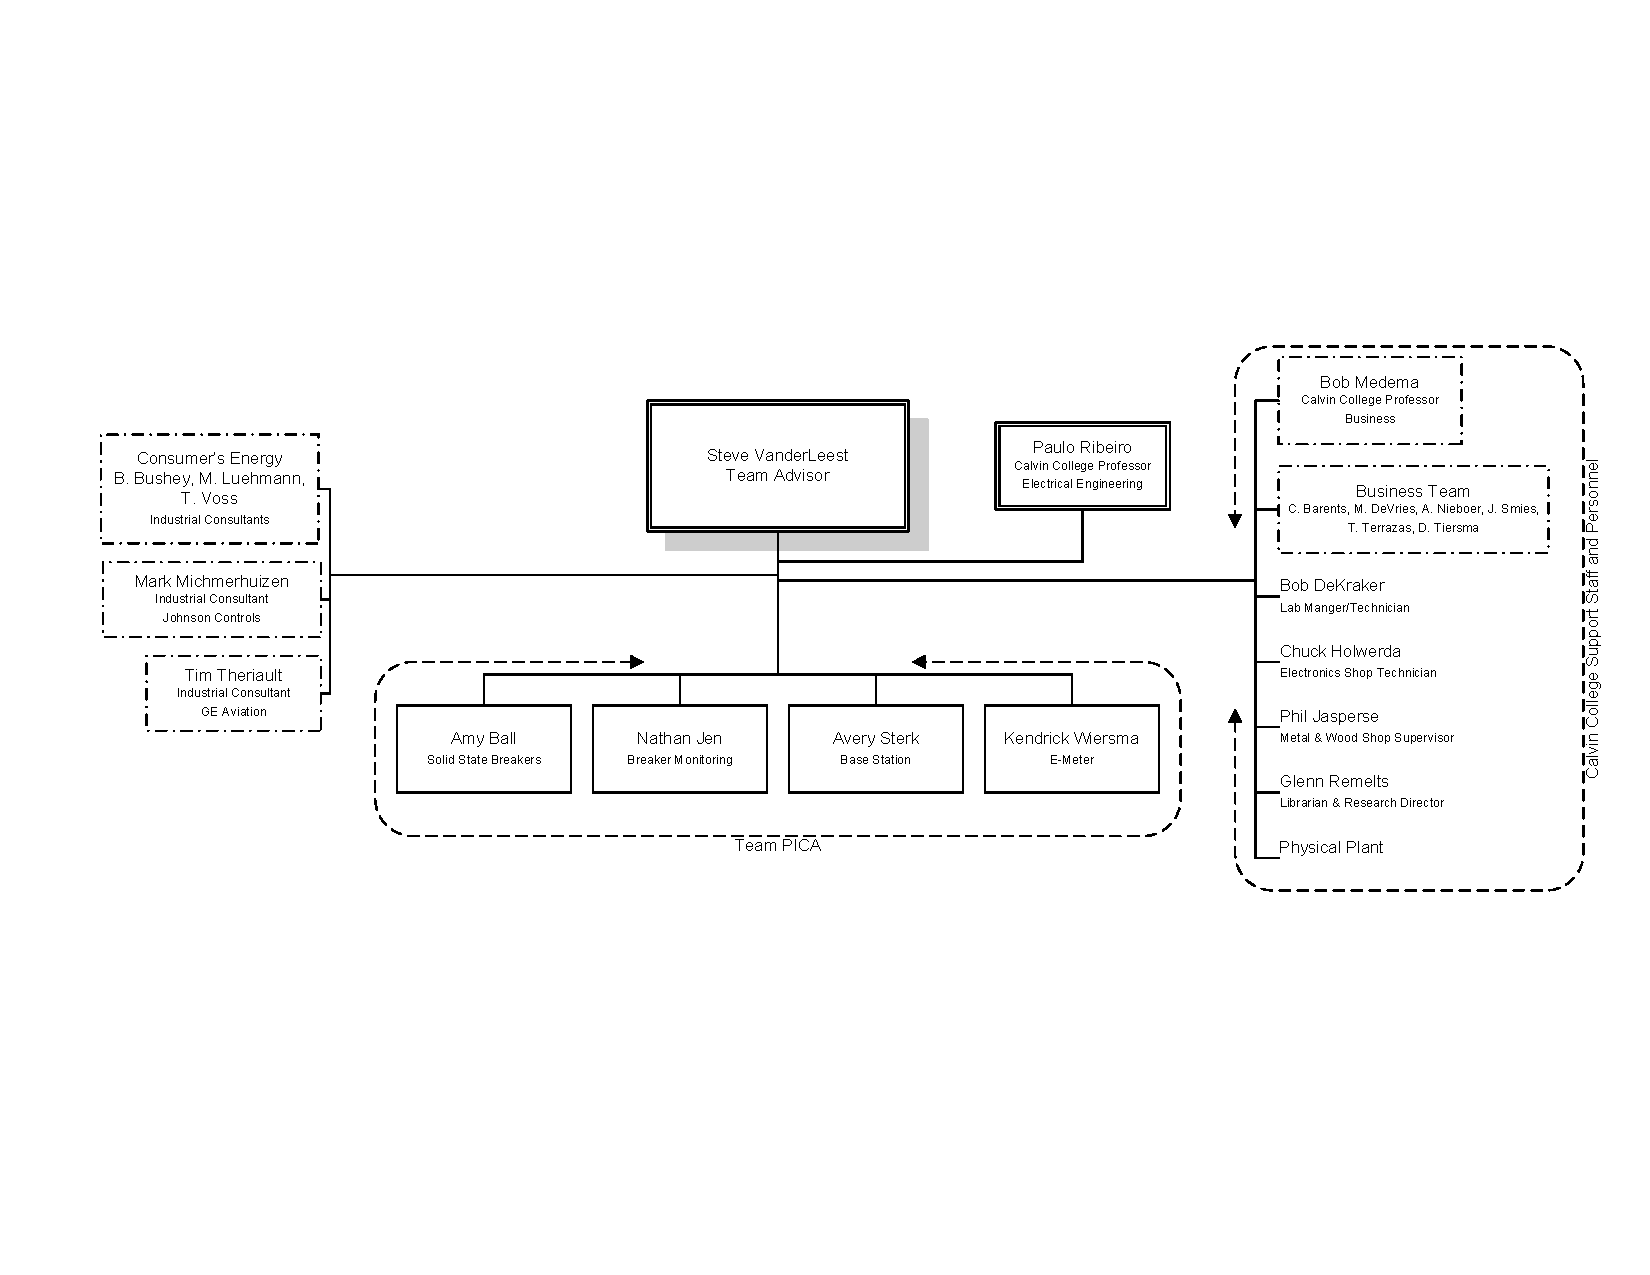
\includegraphics[width=6.5in]{figures/TeamOrgChart}
\caption{Team PICA Organizational chart.}
\label{fig:orgchart}
\end{center}
\end{figure}

\subsection{Team Responsibilities}
\subsubsection{Amy}
Amy, along with Nathan, makes up the hardware part of the team. They are in charge making decisions regarding hardware-specific sections of the project. Amy is also in charge of the Breaker sub-system of the project. She has the most complete understanding of their functions and specific requirements, she may delegate sub-sections to other team members, but she will have a good grasp of how they fit into the larger system. A sub-system of the Breakers is the monitoring section, which the team delegates to Nathan. Nathan and Amy will be working together closely with the full sub-system of the solid-state breakers.

\subsubsection{Nathan}
Nathan is co-leader with Kendrick. They are in charge of scheduling and assigning tasks, scheduling meetings, keeping team on time, on task, and will answer project questions. Nathan, along with Amy, makes up the hardware part of the team. They are in charge making decisions regarding hardware-specific sections of the project. Nathan is also in charge of helping integrate the sub-sections into the whole system, which includes having a detailed, basic understanding of each sub-system, and knowing how each relates to the overall requirements and goals. Nathan is also in charge of the monitoring section of the solid-state breakers.

\subsubsection{Avery}
Avery is in charge of the Base Station section of the project. He has the most complete understanding of it's function and specific requirements. He may delegate sub-sections to other team members, but he will have a good grasp of how they fit into the larger system. He, along with Kendrick, makes up the software part of the team; they make decisions regarding software-heavy sections of the project.

\subsubsection{Kendrick}
Kendrick is in charge of the E-Panel section of the project. He has the most complete understanding of it's function and specific requirements. He may delegate sub-sections to other team members, but he will have a good grasp of how they fit into the larger system. He is also co-leader with Nathan and they will share duties as necessary. He, along with Avery, makes up the software part of the team; they make decisions regarding software-heavy sections of the project.

\subsection{Schedule}
In order to complete the project within the established deadlines, the design team established a schedule and task-oriented deadlines to supplement the larger senior design program-established deadlines. In doing so, the design team selected to address the subsystems individually. The design team will first focus on the solid-state circuit breakers and circuit-monitoring devices, which they hope to complete by the end of the fall semester. The other two subsystems, the base station and the main smart meter, will gain focus in the second semester. Table \ref{Task_list.tex} shows a list of major milestones for the project with the estimated date of completion for each. The chart also shows the number of hours estimated needed for each task and any dependencies. Items in bold indicate tasks scheduled for completion by the current date and labor totals are shown in the bottom right. 

{
\small
\begin{longtable}[c]{|>{\raggedright}b{2in}|>{\raggedright}b{1in}|>{\raggedright}b{1in}|b{0.75in}|b{1in}|}
\caption{Task lists\label{Task_list.tex}}\\
\hline
\rowcolor{lightgray}
Milestone & Estimated Completion & Dependence & Estimated Labor &  \\
\hline
\endfirsthead
\caption[]{Continued from previous page}\\

\hline
\rowcolor{lightgray}
Milestone & Estimated Completion & Dependence & Estimated Labor &  \\
\hline
\endhead
\multicolumn{5}{r}{{Continued on next page}} \\
\endfoot

\endlastfoot
Project scope and functionality determined & Oct 25, 2010                                & none                      & 40  &              \\\hline
Project goals and requirements set         & Nov 16, 2010                                & Scope and functionality   & 60  &              \\\hline
Design criteria determined                 & Nov 19, 2010                                & Goals and requirements    & 15  &              \\\hline
Preliminary breaker design set             & Nov 23, 2010                                & Criteria                  & 50  &              \\\hline
Preliminary e-meter design set             & Feb 2, 2010                                 & Criteria                  & 50  &              \\\hline
Preliminary base station design set        & Mar 6, 2010                                 & Criteria                  & 50  &              \\\hline
Breaker prototyped and tested              & Dec 1, 2010                                 & Design set                & 30  &              \\\hline
E-meter prototyped and tested              & Feb 13, 2010                                & Design set                & 30  &              \\\hline
Base station prototyped and tested         & Mar 19, 2010                                & Design set                & 30  &              \\\hline
Full system integration                    & Apr 17, 2010                                & All subsystems prototyped & 40  &              \\\hline
PPFS turned in                             & Dec 7, 2010                                 & Criteria                  & 130 &              \\\hline
Project presented                          & May 16, 2010                                & Prototyped                & 40  &              \\\hline
                                           &                                             &                           & 325 & 1st Semester \\\hline
                                           &                                             &                           & 240 & 2nd Semester \\\hline
                                           &                                             &                           & 565 & Total        \\\hline
\end{longtable}
}



While subsystems should be able to be completed independent of each other, the design team decided to address the circuit-by-circuit monitoring component of the project first because of its application to control systems. As members of the design team are taking a class in control systems during the fall semester, working on the breakers while also learning control theory seemed to create an advantageous symbiosis between working and learning. The control systems course also seeks to use aspects of the senior design project as learning experiences, so the motivation to combine the controls assignment and the breaker modules is twofold.

The design team has assembled its internal schedule into Gantt chart to show the deadlines of tasks and the linkages between different tasks. Despite having this planning tool and list of tasks, the actual flow and completion of work is frequently different from originally expected. This is partially due to unexpected emergence of assignments and deadlines for the design project itself, but other classes also contribute unforeseen and time-consuming work that impedes progress in the project. To deal with outside deadlines and work, the team tried to think of deadlines focus on work and deadlines to two or three weeks out. Team members were encouraged to think in general terms only about deadlines more than a couple weeks out to help keep focus on current progress. As the semester progresses, these emergent due-dates should decrease in number and severity, allowing the design team to devote more time to the project.

In order to complete the project, the team needs to accomplish a variety of tasks shown in the work breakdown structure below. Much of the early work includes a lot of paperwork outside of the actual design of the system. This includes determining exactly what problem the team is addressing and the requirements needed to solve it. Project goals and design criteria also make up some of the pre-design work. In industry, the customer would already have set many of these requirements, goals and criteria, so to make the project as `real-world-like' as possible, the team put these before the design stage of the project. To make the requirements and goals realistic, the team decided to meet with a variety of professionals in fields including marketing, business and engineering in addition to potential customers. 

Once the project goals, requirements and criteria are set, the team can begin some preliminary design. As another way to limit the project and keep it from getting out of control, the project scope needs to be determined early in the project. A big factor in setting the scope is making the system unique from products that solve similar problems. The first step the team would like to take is to determine the basic functionality of both systems and subsystems and set up functional block diagrams to show this. After the basic functions of each of the subsystems are determined, the team will explore various solutions through general research and trade studies. When the team has compiled a number of different solutions, they can start to eliminate possibilities based on criteria established earlier. To assist with this, the team will use design matrices and comparison tables as visual aids.

After narrowing down the possible solutions, the team will begin the design and implementation stage. Further criteria may include power efficiency, cost of building the system, and availability of components. As  design aspects apply to all subsystems, and since development of the subsystems will occur at different rates as mentioned earlier, the finalized designs will not finish simultaneously. Testing will occur after designing and building the various parts of the subsystems. The team decided that the breakers, breaker monitors, main system monitor and wireless communication should be the first parts of the system completed. Other parts that will require finalization and building include the upgrade mechanism, base station, display module and firmware. Each of the parts will require modifications based on the testing results. Modifications to each of the parts may be necessary based on the testing results, so this section may take multiple iterations before it is complete.

Assembly of the full system will follow the individual parts' completion, along with testing for a variety of things. Some specific things the team hopes to include in the testing are tests based on outside criteria, tests based on requirements set by the team and testing common possible failure points. As the team is working with a limited amount of time that may not allow for full testing of the system, some of the long term testing procedures including accelerated lifetime testing will be written up for later use outside of the class.

Communication will be critical to the success of the project, both during and after so the team aims to provide documentation of all design decisions and testing done throughout the year. As the customer will need to interact with the system effectively, the team hopes to provide a user manual as well. For the class, the team needs to present the project on a number of occasions and hopes to demonstrate their work to all groups associated with the project, including business groups, customers and technical professionals.


